\begin{minipage}[t]{180mm}
\fcolorbox{black}{white}{
\begin{minipage}[b]{30mm}

\includegraphics[width=0.5\linewidth]{unflogo.pdf}
\end{minipage}
\begin{minipage}[b]{100mm}
\Huge \textbf{UNF NEWZ} \\
\Large -- Søvn og retsstavning er overvurderet! 
\end{minipage}
\begin{minipage}[b]{50mm}
\Large Onsdag 17.07.2015 \\
\normalsize Redigeret i \LaTeX\ af \\ SOM, MGS, MMN, SABH
\end{minipage}
}
\end{minipage}



\begin{minipage}[b]{0.95\linewidth}
\begin{minipage}[t]{0.47\textwidth}
\vspace{1mm}
X
\vspace{-7mm}

\section*{Fakta om Jylland}
JYLLAND er i virkeligheden en forkortelse for Jernalderens Yderst Lovlige og Legitime Arbejderes Nydannede Danmark.

\vspace{-3mm}

\section*{Ninjas dagbog}


{\flushright\emph{Ninja, næsten glad}}

\vspace{-3mm}
\section*{Madanmeldelse -- Kaffe}
\fcolorbox{black}{white}{$\aleph_4$ ud af $\aleph_3$ chokoladekiks}


\end{minipage}%
\hfill\begin{minipage}[t]{0.47\textwidth}
\vspace{2mm}
\section*{Vejrudsigt}
\textbf{IMF, AU (fra DMI)}: Temperaturer fra 14 til 23 grader og tørvejr med en del sol indtil midt om eftermiddagen. Der forventes et moderat antal græspollen, og et lavt antal birkepollen.

\textbf{SEN/ASN}: Solskin og 26 grader, men nogle skyer. Luftfugtighed på cirka 90 \% og ingen vind.

\vspace{-2mm}
\section*{Dagens inegnør}

\vspace{-4mm}
\section*{Dagens sandsynlighed}
Sandsynligheden for at få nok søv på Mat-Camp er $0$.

\vspace{-4mm}
\section*{Ikke-kommutativ studenterrådgiv.}
\emph{Kære brevkasse}
 
\emph{Hilsen, en fortvivlet arrangør}

\vspace{-1mm}
\subsection*{Svar}

{\flushright\emph{Hilsen den ikke-kommutative studenterrådgivning}}

\vspace{1mm}
%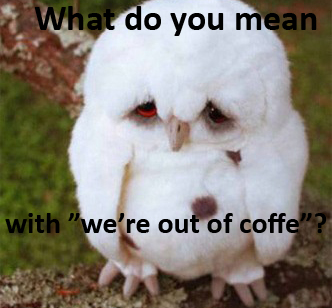
\includegraphics[width=\linewidth]{coffee-ugle2.jpg}
\vspace{-3mm}
\end{minipage}

\begin{center}
\tiny UNF Newz er avisen hvor at ansvarshavende redaktør fralægger sig ethvert ansvar for eventuel plagiering, kaniner, tysk, stavefelj, kaffe, dårlig humor, glemsomhed, katte, store sigmaer, pile, skyer, dårlige oversættelser og alt hvad eventuelle homo sapiens sapiens kunne finde på at holde imod UNF Newz! Dog tager UNF Newz fuld credit og copyright for alle guldkorn, magickort, mus, \TeX, humor, smil, Mortener, kaffe, før-fremtid, ringe og/eller rubik's cube.
\end{center}
\end{minipage}

